\section{nRF24L01}
The following section contains the tests performed on the nRF24L01 radio module. These tests were performed to determine how 

\subsection{Range}
A basic test to test the range is useful to ensure that the module is usable in a practical application with a wide distance between units.

Testing is done by having two units set as transmitter and reciever units respectively, having the transmitter transmit a single signal repeatedly while increasing the distance between the units. When the reciever no longer recieves the signal, the distance can then be measured.

This tests showed a range of about 160 meters with no obstacles, though the number of packets succesfully transmitted without errors lowered the longer the distance.

\subsection{Bit Error Rate}
When transmitting data from one unit to another, knowing that the data is correct is important. To get an idea of how much error is introduced in the communication, a bit error test can be performed, known as BERT from this point on.

\subsubsection*{About BERT}

The basic concept of BERT is to send a known datastream from one unit to another, and check how much it differs from the expected datastream.

The duration of a BERT should vary depending on the results. To get an exact result it would have to take an infinite amount of time, which of course is not feasible. But due to the nature of randomness, if only a small amount of errors are met, then it could just be a "lucky" test, so the testing length would have to be sufficiently long for getting a general idea.

Because of this, multiple BERT runs was executed.

\subsubsection*{Executing BERT} 
The test was executed by sending packets from an Arduino to a Raspberry Pi, using the nRF24L01 modules.

The code running on the devices for the test can be found in Appendix \ref{cha:bertcode}.
The sender code transmits some deterministic value, and the receiver checks whether the received packet is the same as the one expected. If the two packets match, the 'successes' value is incremented, if not, the 'errors' value is incremented.

The BERT was executed four times. The first three times with 1.000.000 packets transmitted, and the fourth time with 10.000.000 packets. For every 1.000 packet received, the number of errors and successes were printed for those 1.000 packets. 
The values were then imported into a spreadsheet for statistics.

The complete spreadsheet with results and graphs can be found on the attached DVD. 

\subsubsection*{Result of BERT}
The results of the BERT showed a packet failure under one percent. Some spikes were present in the test results, with the highest being at 797 missed packets, which occured in the first test, as seen in figure \ref{fig:bert1}.

\begin{figure}[h!]
\hspace*{-2cm}
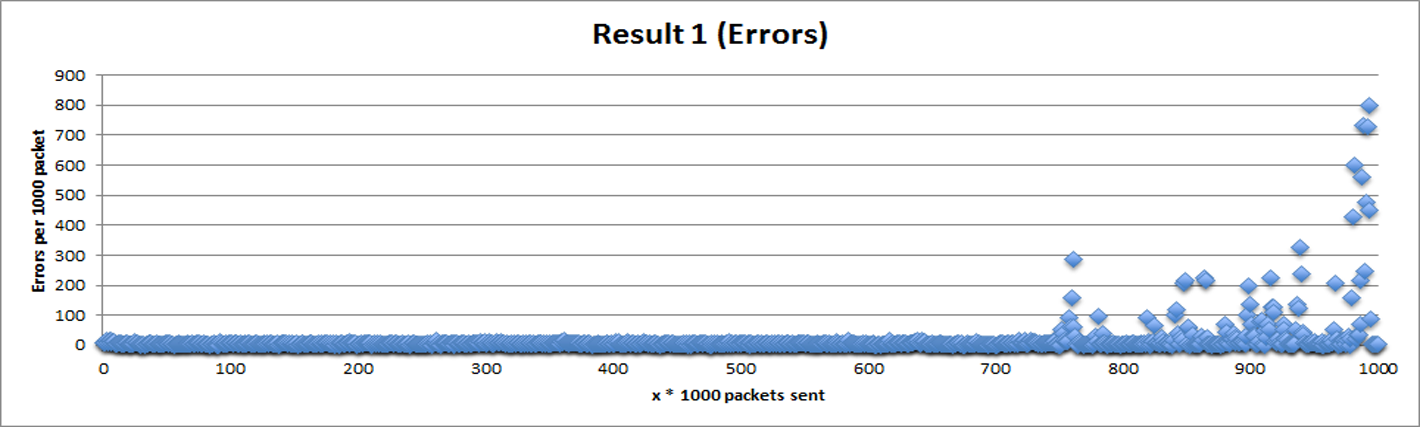
\includegraphics[width=1.3\textwidth]{chapters/test/figures/res1.png}
\caption{Graph representing the first BERT run.}
\label{fig:bert1}
\end{figure}

The three last tests generally had a lower number of missed packets. Test number two had a peak of 304 lost packets [Figure \ref{fig:bert2}], test three had a peak of 340 lost packets [Figure \ref{fig:bert2}] and test four had a peak of 163 lost packets [Figure \ref{fig:bert3}].

\begin{figure}[h!]
\hspace*{-2cm}
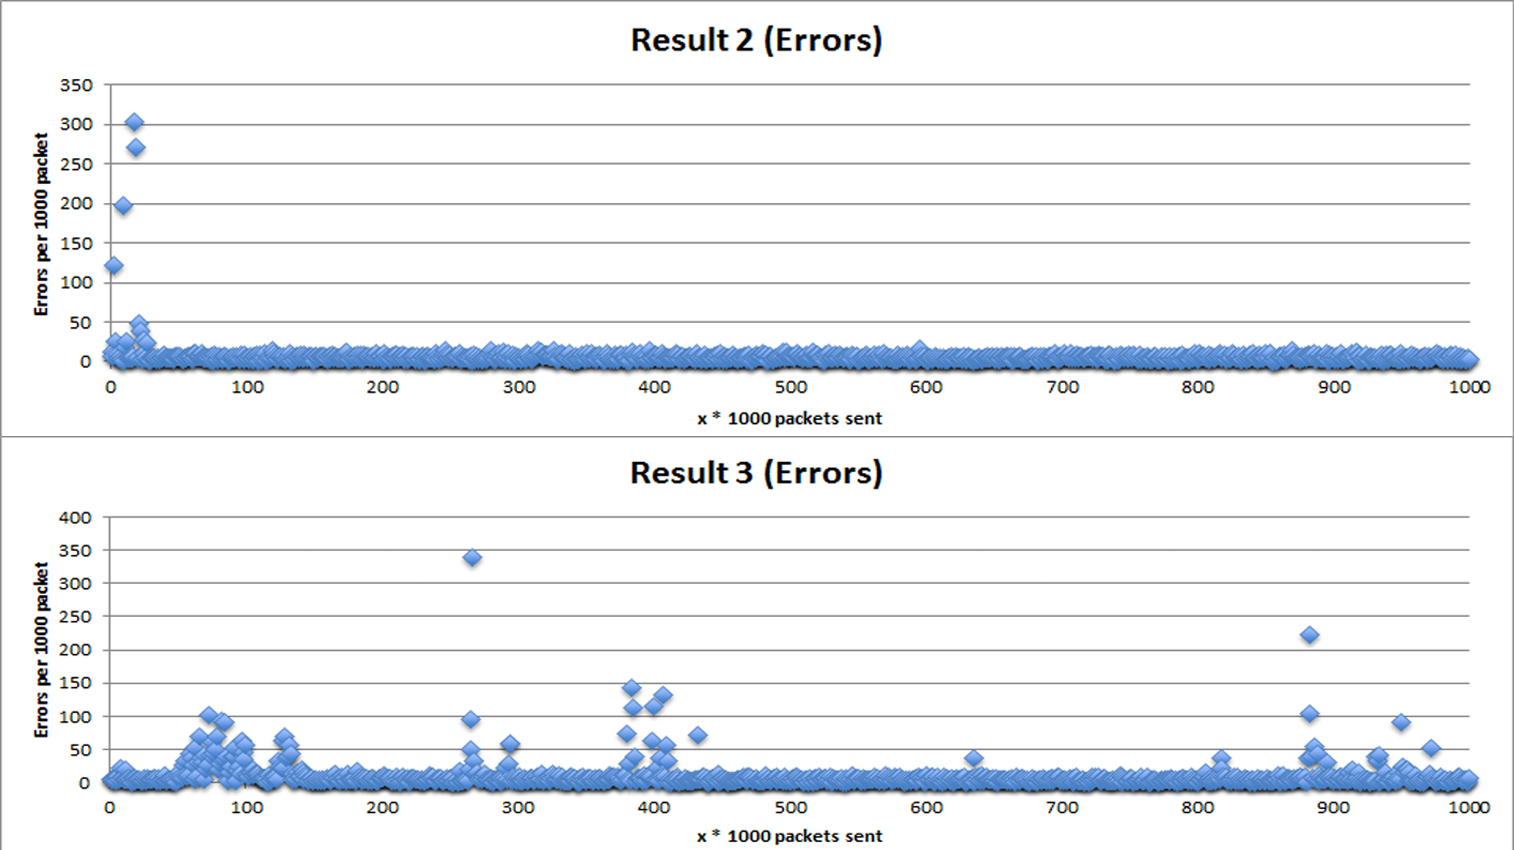
\includegraphics[width=1.3\textwidth]{chapters/test/figures/res5.png}
\caption{Graph representing the second and third BERT run.}
\label{fig:bert2}
\end{figure}

As seen on the first and second test[Figure \ref{fig:bert2}], the high number of errors occured in clusters. This could be attributed to the time of the testing, where other groups might have been testing, or some other source of interference occurred.

Most of the tests were high in successes, and low on failures. In the first run, the average failed packets per 1.000 was at 16.5. The second run had an average of 6.4 failed per 1.000. Third run had 9.3 failed per 1.000 and the fourth run had 7.2 failed per 1.000.


\begin{figure}[h!]
\hspace*{-2cm}
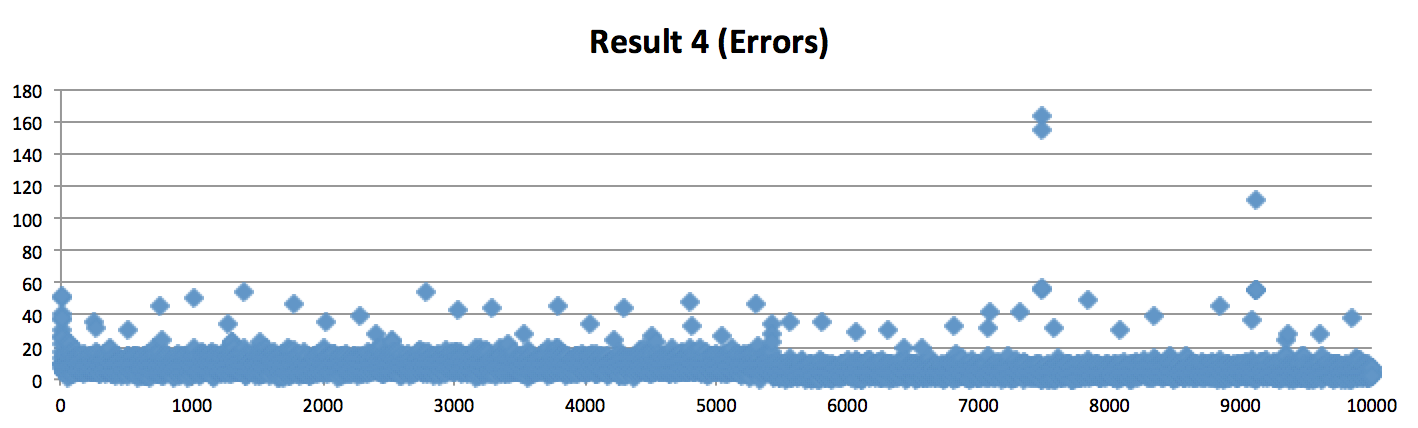
\includegraphics[width=1.3\textwidth]{chapters/test/figures/res4.png}
\caption{Graph representing the fourth BERT run.}
\label{fig:bert3}
\end{figure}

The fourth run was performed using ten million packets, and the graph provides better insight on the randomness of errors. A few spikes appeared, but usually smaller spikes between 40 and 60 packets lost per 1.000.

Generally, the error count is low, and even with the spikes the module seems stable. On a golf course, there will not be the same level of interference as in the group room, surrounded by wireless networks, phones, bluetooth and other sources of interference.

%primarysource http://www.radio-electronics.com/info/rf-technology-design/ber/bit-error-rate-testing-bert.php
